\documentclass[hyperref={pdfpagelabels=false}]{beamer}
\author{Vajna Mikl\'os (AYU9RZ), Veres-Szentkir\'alyi Andr\'as (YZIOAW)}

\setbeamertemplate{background canvas}[vertical shading][bottom=white,top=structure.fg!25]

\usetheme{Warsaw}
\setbeamertemplate{headline}{}
\setbeamertemplate{footline}[page number]
\setbeamersize{text margin left=0.5cm}
  
\usepackage[magyar, english]{babel}

\usepackage{times}
\usepackage[utf8]{inputenc}
\usepackage[T1]{fontenc}

\begin{document}

\title{Szoftverarchitektúrák (VIAUM105)\\Egyszerű verziókövető rendszer}
\date{2010. december 7.}

\frame{\titlepage}

\begin{frame}
\frametitle{Bevezető / Megvalósítandó feladat}
\begin{itemize}
\item Verziókövető rendszer SQL scriptek számára
\item Felhasználó letölti, létrehozza helyben a sémát, módosítja
\item Ha készen van, CREATE SCRIPT és feltölti
\item Optimista (3-way merge) és pesszimista konkurencia-kezelés (lockolás)
\item Operációk: létrehozás, törlés, letöltés, frissítés, zárolás, történet
\item Jogosultságok: felhasználó és adminisztrátor
\end{itemize}
\end{frame}

\begin{frame}
\frametitle{Választott technológiák / szempontok}
\begin{figure}[H]
\includegraphics[width=15mm,keepaspectratio]{layers.pdf}
\end{figure}
\begin{itemize}
\item Architektúra: háromrétegű
\item Programnyelv: C++
\item Verziókezelő: Git - elosztott
\item Platformok: Linux, Windows (kliens) - hordozhatóság
\item Dokumentáció: Doxygen, \TeX{} - verziókezelés könnyű
\item Keretrendszerek: cppunit, omniORB, Qt - biztonság, megjelentés
\item Adatbázis: SQL (MySQL)
\end{itemize}
\end{frame}

\begin{frame}
\frametitle{Adatelérés}

\begin{figure}[H]
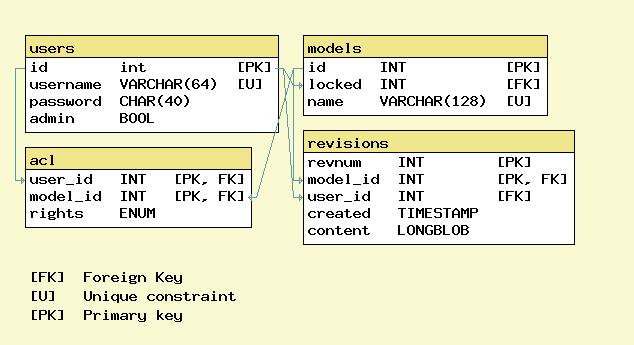
\includegraphics[width=75mm,keepaspectratio]{sqlschema.png}
\end{figure}

\begin{itemize}
\item QtSql - mint JDBC Java esetén
\item Jelenleg MySQL, de driver lecserélése csak beállítás kérdése
\item Tranzakciók
\item Biztonság: prepared statementek
\item Constraintek - cascade-ek
\item Triggerek - revnum beállítás
\end{itemize}
\end{frame}

\begin{frame}
\frametitle{Üzleti logika}
\begin{itemize}
\item IDL interfész mögé rejtve
\item omniORB használata
\item Öröklések megkerülése: tie classok
\item Interfészekhez több implemntáció (Model - ModelWriter, ModelReader)
\end{itemize}
\end{frame}

\begin{frame}
\frametitle{Üzleti logika - interfészek}
\begin{figure}[H]
\includegraphics[width=60mm,keepaspectratio]{classdiagram.pdf}
\end{figure}
\end{frame}

\begin{frame}
\frametitle{Megjelenítési réteg}
\begin{itemize}
\item Qt használata - QSettings
\item IDL interfészt használja omniORB-vel
\item Natív megjelenés
\item Átméretezhető ablakok
\end{itemize}
\end{frame}

\begin{frame}
\frametitle{Tesztelés}
\begin{itemize}
\item cppunit használata
\item A testsuite elindítja a corba servert
\item Minden testcase előtt adatbázis reset
\item Végén corba server leáll
\item 39 testcase
\end{itemize}
\end{frame}

\begin{frame}
\frametitle{Dokumentáció}
\begin{itemize}
\item Követelmény specifikáció
\item API dokumentáció - Doxygen, többi \TeX{}
\item Rendszerterv (fejlesztőknek, ami nincs az API dokumentációban)
\item Telepítési dokumentáció
\item Felhasználói dokumentáció
\item Prezentáció
\end{itemize}
\end{frame}

\begin{frame}
\frametitle{Telepítés}
\begin{itemize}
\item Kiszolgáló: Debian csomag
\item Kliens: Debian csomag, NSIS installer Windowsra
\item Installer készítése is hordozható
\item Automatizált build környezet
\end{itemize}
\end{frame}

\begin{frame}
\frametitle{Összefoglalás}
\begin{itemize}
\item Egyszerű verziókezelő rendszer háromrétegű architektúrával
\item SQL, CORBA és Qt alapon
\item Automatizált tesztelés
\item Automatizált API dokumentáció
\item Automatizált installer készítés
\end{itemize}
\end{frame}

\end{document}
